\documentclass[letterpaper, 10pt]{report}

% administrivia
% (fold)
\usepackage[utf8]{inputenc}
\usepackage[T1]{fontenc}
\usepackage[english]{babel}
\usepackage[nottoc, numbib]{tocbibind}
\usepackage{hyperref}

% alt dette for ett eksempel
\usepackage[footnotesize, bf, hang]{caption}
\usepackage{subcaption}
\usepackage{floatrow}
\usepackage{calc}
\floatsetup{ 
	heightadjust=object,
	valign=t
}
% (end)

% layout
% (fold)
%\usepackage{fullpage}
\usepackage[sc]{mathpazo}
\usepackage{inconsolata}
\usepackage[protrusion=true,expansion=true]{microtype}
\usepackage{hyperref}
\usepackage{enumitem}
\usepackage{setspace}
\onehalfspacing
\frenchspacing
\usepackage{listings}
\lstset{
	basicstyle=\ttfamily\footnotesize,
	tabsize=2, 
	breaklines=true
}
\usepackage{wrapfig}
\usepackage{graphicx}
% mindre tekst for sitater
\let\quoteOLD\quote
\def\quote{\quoteOLD\small}
\usepackage[bottom]{footmisc}
% (end)

% citation
% (fold)
\usepackage[
	style=authoryear, 
	backend=bibtex, 
	dateabbrev=false
]{biblatex}
\addbibresource{references.bib}
\DefineBibliographyStrings{english}{%
	urlseen = {Retrieved},
}
% (end)

% front matter
% (fold)
\title{\Huge \textbf{Measuring Productivity in the Software Engineering Industry}}
\author{
	Håkon S. Mork \\ 
	ORGB 423 --- Human Resources Management \\ 
	McGill University \\
	\\
	\emph{With kind contributions from Solfrid Skilbrigt}
}
\date{\today}
% (end)

\begin{document}
\pagenumbering{roman}
\maketitle

% TODO alt
\begin{abstract}
% (fold)
Lorem ipsum dolor sit amet, consectetur adipisicing elit, sed do eiusmod tempor incididunt ut labore et dolore magna aliqua. Ut enim ad minim veniam, quis nostrud exercitation ullamco laboris nisi ut aliquip ex ea commodo consequat. Duis aute irure dolor in reprehenderit in voluptate velit esse cillum dolore eu fugiat nulla pariatur. Excepteur sint occaecat cupidatat non proident, sunt in culpa qui officia deserunt mollit anim id est laborum.
% (end)
\end{abstract}

\tableofcontents

\chapter{Introduction}
\pagenumbering{arabic}

% TODO alt
\section{Objectives}

\section{Company}
% (fold)
Steria is a multinational company founded in 1969 that specializes in information technology consulting, services and management. 
With headquarters in Paris and French administration, Steria is present in 16 countries and on three continents. 
The company boasts more than 20,000 employees and a 2011 annual revenue of €1.75 billion \parencite{steria:stats}.
% (end)

% TODO endre bilde avhengig av endelig layout
\section{Human Resources Professional}
% (fold)
\begin{wrapfigure}{r}{0.3\textwidth}
	\centering
	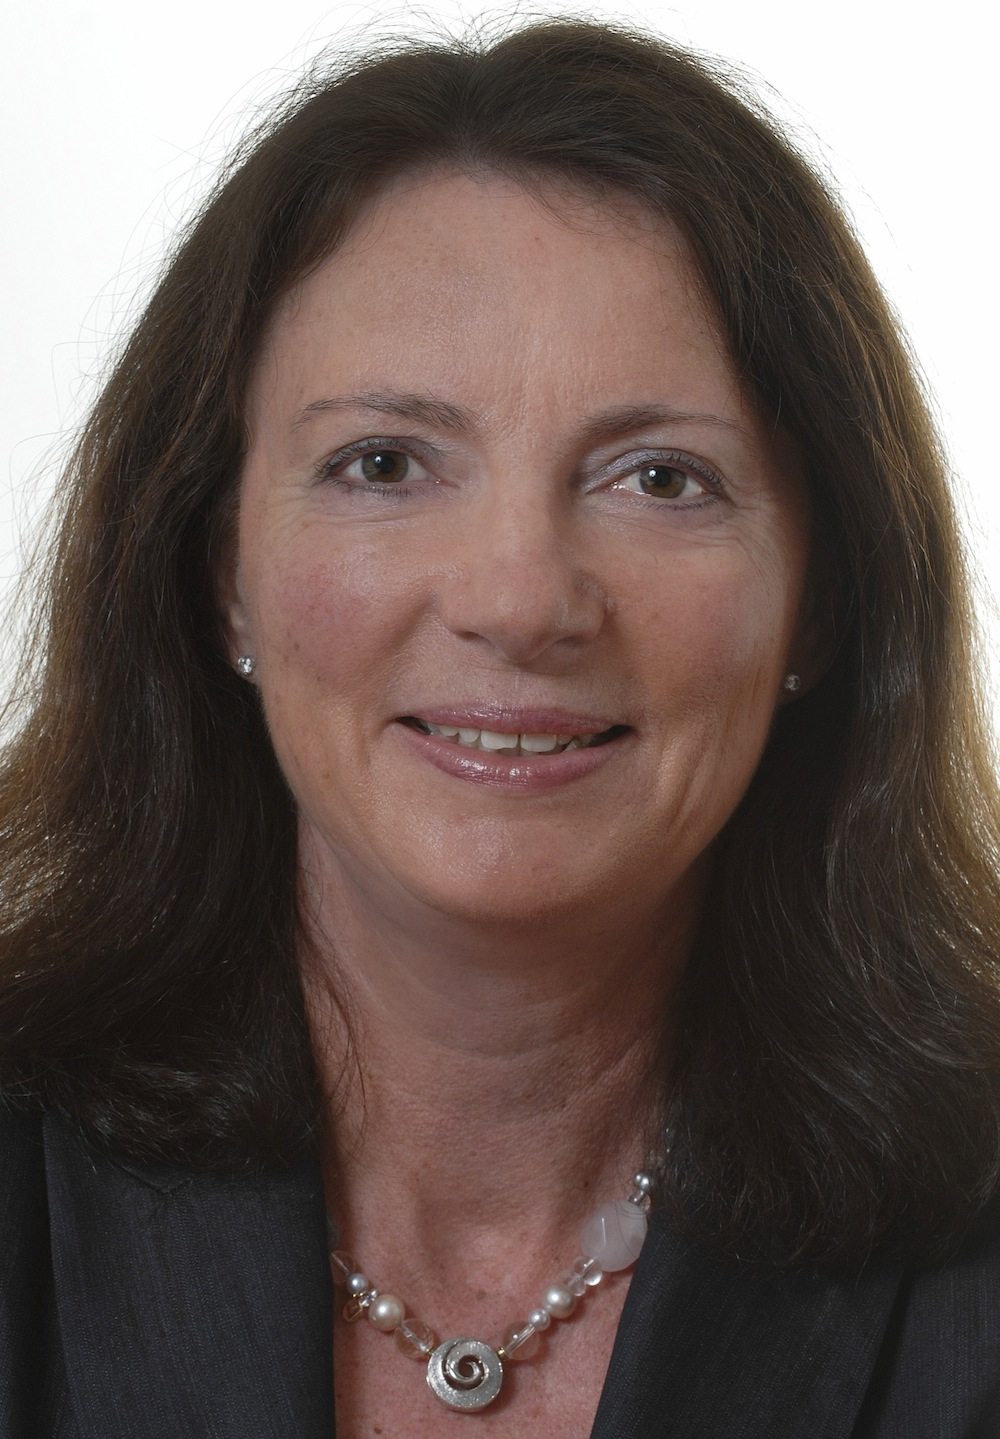
\includegraphics[width=\textwidth]{solfrid}
	\caption*{Solfrid Skilbrigt}
\end{wrapfigure}
Solfrid Skilbrigt, Human Resouces Director of the Norwegian and Scandinavian branch and Deputy CEO of Scandinavia, has kindly agreed to answer my questions about human resource management in her firm. 
A graduate of the University of Trondheim, she has long and varied experience in the fields of information technology, sales, and human resources.

Her accomplishments include leading the company's employer branding, recruitment, and management and organizational development programs, as well as playing a key part in Steria's advancement to being one of the world's leading IT consulting firms. 
Skilbrigt has also been in charge of Steria's global CSR efforts since 2008.

% (end)

% TODO alt
\section{Topic Area}



\chapter{Results and Discussion}

% TODO kompleksitet, mer om basics
\section{Basics of Software Engineering}
% (fold)
Software is unlike any other kind of manmade product. 
It is intangible, complex, and most of its users have no idea how it works; as science fiction author Arthur C. Clarke said, ``Any sufficiently advanced technology is indistinguishable from magic'' \parencite{about:clarke}.
The industry that produces software is also unlike any other, producing incorporeal goods at great cost that XXX.
The economics of software are also peculiar: the cost of producing large-scale software is exorbitant, but having completed it, all subsequent copies can be produced at zero cost. 

How, then, should one measure employee productivity, when the 

not physical, not bound by laws of nature

arbitrary complexity
% (end)

% TODO alt
\subsection{The Development Process}
% (fold)
planning

design

coding (compiling, debugging)

maintenance
% (end)

% TODO complexity, legacy systems
\subsection{Complexity}
% (fold)
Software, unlike virtually any other product, can be in theory be made arbitrarily complex and full-featured.

increasing over time

systems are rarely made from scratch anymore, more often upgrading, patching and tinkering on old systems

``legacy'' systems

programmer ability to handle complexity and abstraction is key
% (end)

% TODO alt
\section{Challenges of Measuring Productivity}
% (fold)
individual efforts as part of TQM

\cite{fowler:cannotmeasure}
\begin{quote}
Productivity, of course, is something you determine by looking at the input of an activity and its output. 
So to measure software productivity you have to measure the output of software development---the reason we can't measure productivity is because we can't measure output. 
This doesn't mean people don't try. 
\end{quote}

% (end)

% TODO alt
\subsection{Group Effort}
% (fold)
no lone wolves

how to assess individual contributions to team efforts

who gets the credit when a problem is solved jointly: all? some? in that case, who?
% (end)

% TODO nok om specs nå?
\subsection{External Factors}
% (fold)
One of the perennial problems of the software industry is that neither the maker nor the clients have a precise idea of what the finished product should be like, leading to costly delays as the customer changes their mind and new requirements are added or amended even while the system is being built.
One might think that fixing this problem should be an easy matter; after all, most other engineering disciplines do not face cost overruns of the same order of magnitude that plague the software engineering trade---apart from, perhaps, construction. 
Indeed, early processes and management models used from the mid-20th century onward, when computing was in its infancy, often took cues from the product development processes used in manufacturing REFERENCE, expecting that the process of producing software would be essentially similar to producing any other type of product.

changing specs make life difficult

% (end)

% TODO dual displays, the zone
\subsection{Working Conditions}
% (fold)
\textcite{spolsky:list} argues that disruption is highly damaging to programmer productivity:
\begin{quote}
If a coworker asks you a question, causing a 1 minute interruption, but this knocks you out of the zone badly enough that it takes you half an hour to get productive again, your overall productivity is in serious trouble. 
If you're in a noisy bullpen environment like the type that caffeinated dotcoms love to create, with marketing guys screaming on the phone next to programmers, your productivity will plunge as knowledge workers get interrupted time after time and never get into the zone.
\end{quote}

especially bad for programming because...

% (end)



% TODO litt blabla på begynnelsen
\section{Quantitative Measures}
% (fold)
many measures are easy to quantify


% (end)

% TODO mostly done, review and rewrite
\subsection{Lines of Code}
% (fold)
Measuring employee productivity in terms of number of computer code lines written is a simple, widely used metric REFERENCE. 
However, it is also easily manipulated, often irrelevant or misleading and not a good indicator of individual productivity.

structuring code into reusable parts is widely considered to be best practice; that is, not duplicating code that is similar or identical but instead grouping it together

A further argument against using code line count is that it often has no bearing on the functionality of the program \parencite{albrechtgaffey:linesofcode}. 
As an example, consider the code snippets in two different programming languages in figure \ref{fig:codelineexample}, both written by the author. 
Both these programs do exactly the same thing: prompt the user for a number, and then display the numbers from 1 up to that number. 
Even so, the one written in the C programming language is four times longer than the one written in the Python programming language. 
Is an employee who writes the longer one four times as productive as someone who writes the shorter one? 
Clearly not, since they both solve the same problem---but while the programmer who wrote the terser version may move on to new problems to solve, the programmer who writes more verbosely takes longer to finish the task, simply because there is more typing to be done. 
In addition, one should take into consideration the extra time spent on debugging the verbose version: 
Much like how a mechanical engineer seeks to minimize the number of moving parts in a machine, a software engineer seeks to write as little code as possible, since everything that is ``moving'' is a potential source of errors and malfunctions. 

% language length example
% (fold)
\newsavebox{\pythonexample}
\begin{lrbox}{\pythonexample}
\begin{lstlisting}
n = int(input())
for i in range(1, n + 1):
	print i
\end{lstlisting}
\end{lrbox}

\newsavebox{\cexample}
\begin{lrbox}{\cexample}
\begin{lstlisting}
#include <stdio.h>
int main(int argc, char **argv) 
{
	int n;
	scanf("%d", &n);
	int i;
	for (i = 1; i < n + 1; i++) 
	{
		printf("%d\n", i);
	}
	return 0;
}
\end{lstlisting}
\end{lrbox}

\begin{figure}
\ffigbox{
	\begin{subfloatrow}
		\ffigbox[\FBwidth+1em]{\usebox{\cexample}}{\subcaption{Example in C}}
		\ffigbox[\FBwidth+1em]{\usebox{\pythonexample}}{\subcaption{Example in Python}}
	\end{subfloatrow}
}
{\caption{These two pieces of computer code, in two different programming languages, do exactly the same thing---yet one is four times longer than the other.}\label{fig:codelineexample}}
\end{figure}
% (end)

This may be a trite observation when discussing the example in figure \ref{fig:codelineexample}, with twelve lines of code instead of three, but the principle is more general. 
Indeed, \textcite{graham:succinctness} argues that terseness is one of the programmer's prime virtues:
``[S]uccinctness is power, or is close enough that except in pathological examples you can treat them as identical.
It seems to me that succinctness is what programming languages are for.''
Thus measuring the number of lines of code an employee writes is at best irrelevant and at worst misleading. 
Still, this metric is widely used, mainly due to the ease with which one can implement an appraisal system based on it. 
Automated tools can easily count the number of code lines written by a single person in a single day, making it easy to track an employee's output over time. 
While the amount of code a single person writes is no solid indicator of their personal productivity, the amount of code that, in total, makes up a project is a decent gauge of the project's size and scope. 
\textcite{fowler:cannotmeasure} argues that

\begin{quote}
I can be pretty confident that a 100 \textsc{kloc}\footnote{Thousand lines of code.} system is bigger than a 10 \textsc{kloc} system. But if I've written the 100 \textsc{kloc} system in a year, and Joe writes the same system in 10 \textsc{kloc} during the same time, that doesn't make me more productive. Indeed, I would conclude that our productivities are about the same, but my system is much more poorly designed.
\end{quote}

On that account, code lines should be used solely as a measure of project size and complexity, not individual productivity.

% (end)

% TODO alt
% se fowler for startpunkt
\subsection{Function Points}
% (fold)
piece of functionality

hard to pinpoint

useful to customer vs. scaffolding and utilitiy functions
% (end)

% TODO cyclomatic, halstead
\subsection{Advanced Metrics}
% (fold)
%http://www.examiner.com/article/article-9-how-to-measure-programmer-productivity
cyclomatic

%http://en.wikipedia.org/wiki/Cyclomatic_complexity
%http://www.literateprogramming.com/mccabe.pdf
halstead
% http://en.wikipedia.org/wiki/Halstead_complexity_measures

% (end)



\section{Qualitative Measures}

% TODO alt
\subsection{Code Quality}
% (fold)
ideally the best option

somewhat subjective

quotes galore up in this

hard to formalize

% (end)

% TODO alt
\subsection{Features Added}
% (fold)
hard to pinpoint who is responsible

not good enough for individual appraisal (important because reference says so)

% (end)

% TODO alt
\subsection{Bugs Removed}
% (fold)
much of programming is correcting the mistakes of others

% (end)

\subsection{Peer Evaluation}



\section{Industry Practice}

\subsection{General Findings}

\subsection{Steria}


\section{Discussion}



% TODO leave for last
\chapter{Conclusion}
% (fold)
no panacea

summarize practices

% (end)

\appendix
% TODO still alle spørsmål!
\chapter{Interview Questions}
% (fold)
\begin{enumerate}[leftmargin=*]
	\item What is your name?
	\item What is your quest?
	\item What is the airborne velocity of an unladen swallow?
\end{enumerate}

% (end)

% TODO still alle spørsmål!
\chapter{Letter of Thanks}


%\nocite{*}
\printbibliography
\phantomsection
\addcontentsline{toc}{chapter}{Bibliography}

\end{document}


%http://www.sei.cmu.edu/library/abstracts/reports/92tr020.cfm
%http://scholar.google.co.uk/scholar?q=lines+of+code&btnG=&hl=en&as_sdt=0%2C5
